\documentclass[10pt,twoside]{scrreprt}

\renewcommand{\textfraction}{0.001}
\renewcommand{\topfraction}{0.999}   
\renewcommand{\bottomfraction}{0.999}

\usepackage{graphicx}
\usepackage{amsmath}
\usepackage{mathtools}
\usepackage{amssymb}
\usepackage[bibencoding=utf8, backend=biber, style=numeric, minbibnames=1, maxnames=5]{biblatex}
\addbibresource{bibliography.bib}
\usepackage{a4,color}
\usepackage{tikz}
\usepackage{calc}

\usepackage{booktabs}
\usepackage{caption}
\usepackage{float}
\usepackage{url}
\usepackage{listings}

\usepackage[T1]{fontenc}
\usepackage[utf8]{inputenc}

\usepackage{mathpazo}

\definecolor{red}{rgb}{1,0,0}
\definecolor{green}{rgb}{0,1,0}
\definecolor{blue}{rgb}{0,0,1}
\definecolor{darkblue}{rgb}{0,0,0.8}

\definecolor{yellow}{rgb}{1,1,0}
\definecolor{lightblue}{rgb}{0,1,1}
\definecolor{magenta}{rgb}{1,0,1}
\definecolor{lightgrey}{rgb}{0.5,0.5,0.5}
\definecolor{grey}{rgb}{0.35,0.35,0.35}
\definecolor{darkgrey}{rgb}{0.2,0.2,0.2}
\definecolor{ockerrot}{rgb}{0.859,0.375,0.152}

% Default fixed font does not support bold face
\DeclareFixedFont{\ttb}{T1}{txtt}{bx}{n}{12} % for bold
\DeclareFixedFont{\ttm}{T1}{txtt}{m}{n}{12}  % for normal

% Custom colors
\usepackage{color}
\definecolor{deepblue}{rgb}{0,0,0.5}
\definecolor{deepred}{rgb}{0.6,0,0}
\definecolor{deepgreen}{rgb}{0,0.5,0}

\usepackage{listings}

% Python style for highlighting
\lstset{
language=Python,
basicstyle=\ttm,
otherkeywords={self, for},             % Add keywords here
keywordstyle=\ttb\color{deepblue},
emph={MyClass,__init__, np},          % Custom highlighting
emphstyle=\ttb\color{deepred},    % Custom highlighting style
stringstyle=\color{deepgreen},
frame=tb,                         % Any extra options here
showstringspaces=false            % 
}


\captionsetup{margin=0pt,font=small,labelfont=sc,labelformat=simple,format=plain,indention=3mm,
 labelsep=endash,textfont=sf,font=sf,singlelinecheck=on,figurename=Fig.,tablename=Tab.}


\fontfamily{ppl}\selectfont

\newcommand*{\bfrac}[2]{\genfrac{\big (}{\big )}{0pt}{}{#1}{#2}}

\begin{document}

\chapter*{Abstract}
\addcontentsline{toc}{chapter}{Abstract}
This thesis studies an algorithms for the detection of circles which are produced by particles travelling through the RICH detectors generating Cherenkov radiation.
At the beginning there is an introduction to the linear hough transform and then to the hough transform to detect circles. The first case considered
is when there is only one unknown (radius) and the center is known. The second case is with two unknowns where the radius is known but the center unknown ($(x,y)$
coordinates of the center are the two unknown parameters).
Lastly there is the case where all the parameters are unkown. For this case there is on the one hand the traditional approach studied with the conventional accumulator
space and on the other hand a new approach is developped and studied. This approach works on the basis that each circle is defined by 3 points. Once there are three
points the radius and the center can be caculated.
	

\chapter{Introduction}
\section{LHC - Large Hadron Collider} % (fold)
\label{sec:lhc_large_hadron_collider}
\begin{figure}[b]
  \centering
  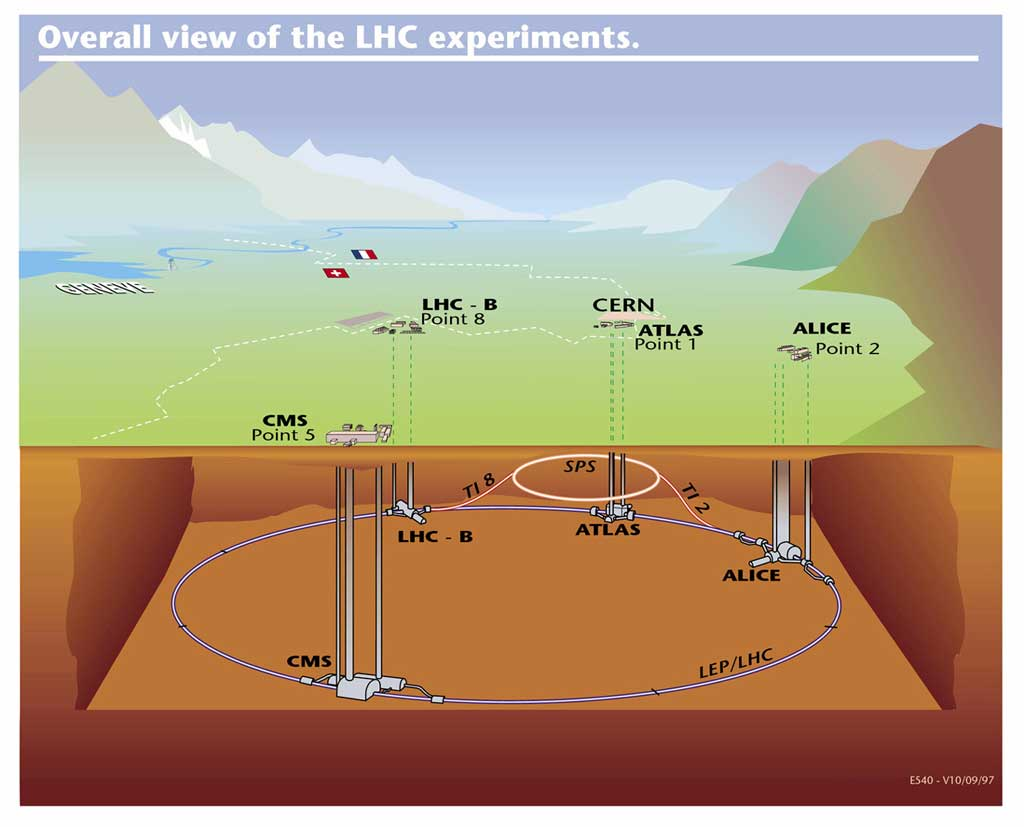
\includegraphics[width=0.6\textwidth]{pics/lhc}
  \caption{The LHC ring with its 4 experiments: ATLAS, CMS, Alice and LHCb}
  \label{fig:lhc}
\end{figure}

The Large Hadron Collider (LHC) is a proton-proton collider. It is the largest and highest-energy particle accelerator in the world. It was built by the European Organisation for Nuclear Research from 1998 to 2008. It aims to test the predictions of different theories in high-energy particle physics, and in particular for the search of the Higgs boson (which has been confirmed this year) and signs for new physics beyong the Standard Model of particle physics. The LHC lies in a tunnel 27\,km in circumference and 100\,m below the surface of the French-Swiss border near Geneva. The LHC was built in collaboration with over 10000 scientists and engineers from over 100 countries. The accelerator has been running with a center of mass energy $\sqrt{s} = 13$ TeV since 20 May 2015.

The LHC hosts four large experiments of which the \emph{LHCb} experiment (Large Hadron Collider beauty) is one. The main goal of the \emph{LHCb} experiment is to study \emph{B}-physics and charm physics such as CP violation and rare decays.



The core physics programm for the period 2014-2015 includes:

\begin{itemize}
  \item <COMMENT: PROGRAM>
\end{itemize}

The fact that at the LHC b-hadrons are predominantly produced in the forward region was used in the construction of the detector. The \emph{LHCb} experiment is a single arm forward spectrometer with a 4\,Tm dipole magnet and a polar angular coverage from 10 to 300 mrad in the horizontal plane (the bending plane of the dipole magnet) and 250 mrad in the vertical plane.


% section lhc_large_hadron_collider (end)

\chapter{LHCb}

An important requirement at LHCb is the particle identification. This is handled by CALO, Muon and RICH sub-detectors. The Calorimeters beside measuring energies and positions of electrons, photons and hadrons also provide indentification of said particles. The Muon system identifies muons to a very high level of purity which is esential for many \(J/\Psi\)'s in their final states.

Hadron identification is very important for decays where the final states of interest are purey hadronic. The LHCb RICH system provides. It is composed of two detectors. One positioned upstream of the dipole magnet and the other one positioned downstream of the dipole magnet. The optics is arranged similarly in both sub-detectors: spherical focusing mirrors project the Cherenkov photons onto a series of flag mirrors which then reflect them onto a series of photon detector arrays, located outisde the detector acceptance~\cite{Powell:2011}.

\begin{figure}[tb]
  \centering
  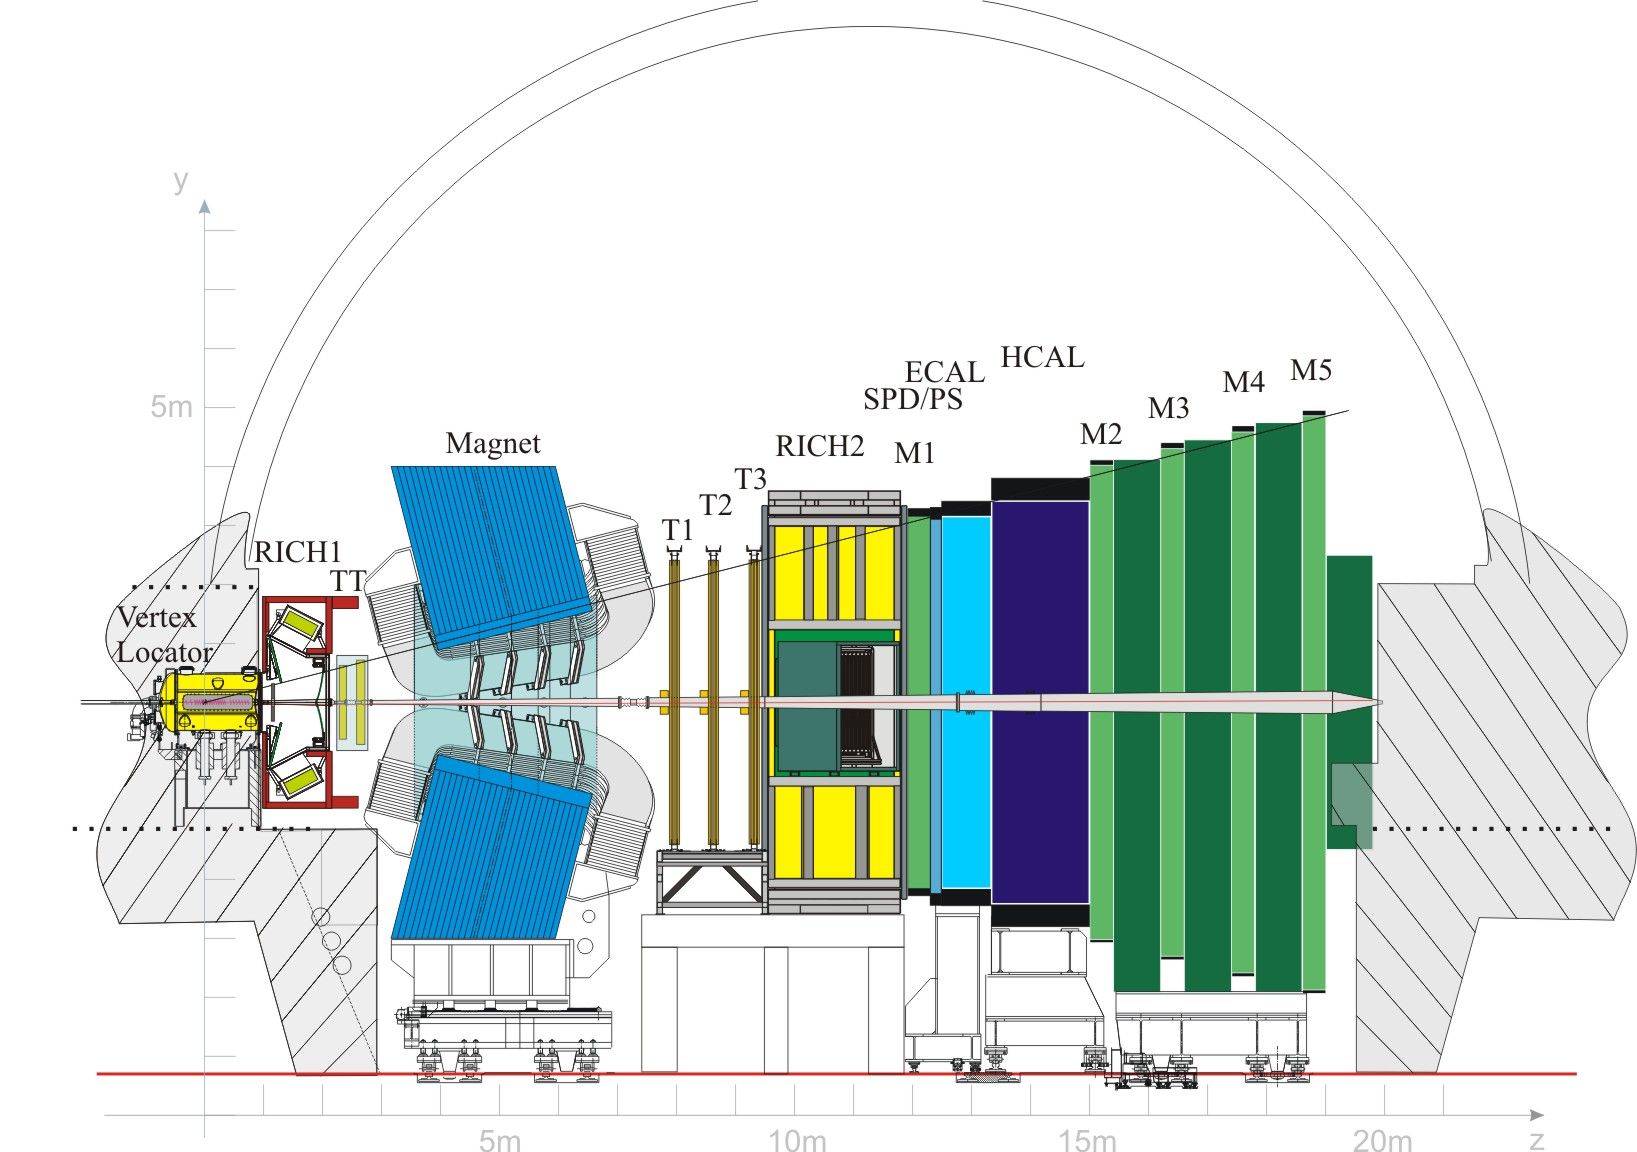
\includegraphics[width=\textwidth]{pics/lhcb_detector}
  \caption{LHCb Detector: RICH1 before the magnet and RICH2 after the magnet with silicon strip detector in between and muon and calorimeter at the end.}
  \label{fig:lhcb}
\end{figure}
\chapter{Theory}

\section{RICH Detector} % (fold)
\label{sec:rich_detector}

Particle identification is a fundamental requirement at the LHCb experiment. Meaningful CP-violation measurements are only possible if hadron identification is available hence the ability to distinguish between kaons and pions is  essential.
The LHCb experiment is unique in the sense that its hadronic particle identification is handled only by the RICH sub-detectors. This means -- as mentioned before -- that the RICH has to cover a wide range of momentum (1-100 $\text{GeV}/c$).

The RICH-1 in front of the magnet covers a lower momentum range from 1-60 $\text{GeV}/c$. It is composed of 5\,cm thick aerogel tiles arranged around the beam pipe. The aerogel with $n=1.03$ is suited for the lowest momentum tracks. Directly behind the aerogel is circa 1\,m of $\text{C}_4\text{F}_{10}$ which covers the intermediate region of momentum.
For the highest momentum tracks, gaseous $\text{C}\text{F}_4$ is used in the RICH-2.

There is a strong corelation between the polar angle and momentum of the tracks. Tracks with a wider angle often have lower momentum. That is why RICH-1 with the aerogel is located before the dipole magnet so tracks with low momentum will be covered before they swept out of the acceptenace by the magnet.

Both sub-detectors are located in low magnetic field regions to keep the tracks straight while they pass through the radiators.

\begin{figure}[tb]
  \centering
  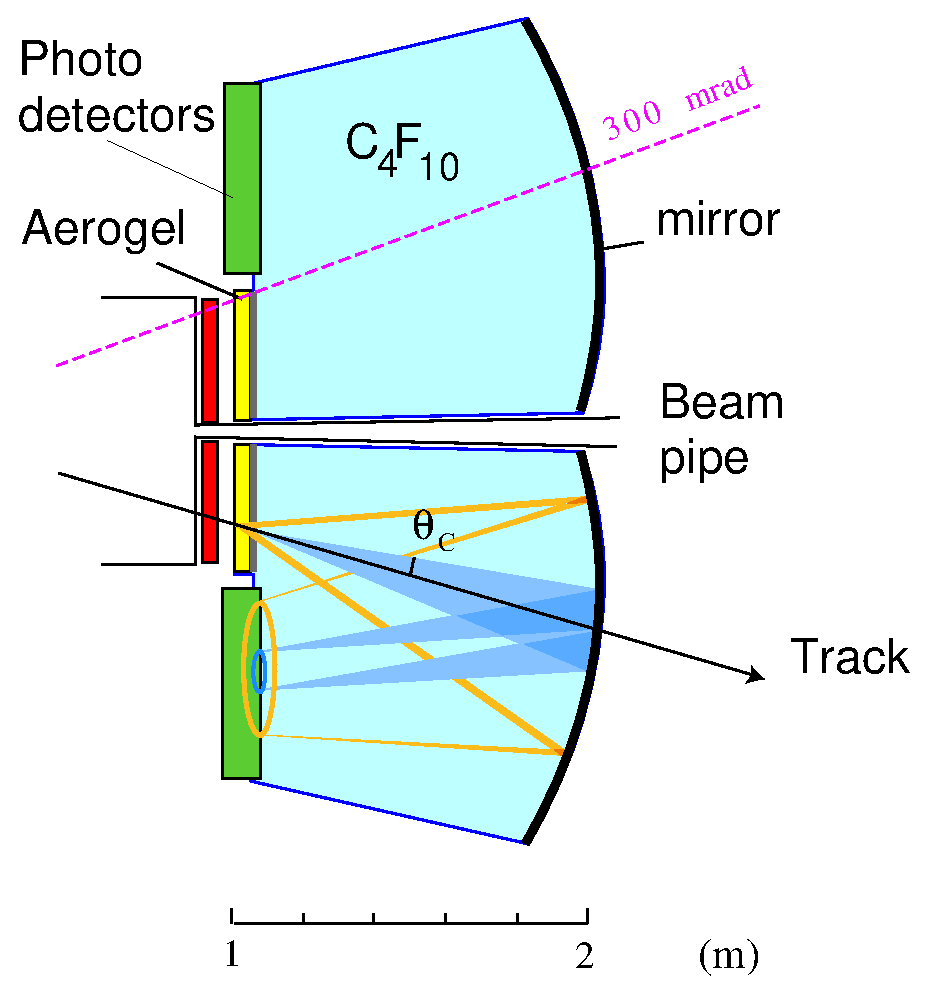
\includegraphics[width=0.5\textwidth]{pics/rich1_schematic}
  \caption{RICH-1 detector \cite{LHCb:2000}.}
  \label{fig:rich1}
\end{figure}
% section rich_detector (end)

\section{Cherenkov-Radiation} % (fold)
\label{sec:cherenkov_radiation}

The speed of light in vacuum, \( \mathbf{c} \), is a universal physical constant. According to Einstein's special theory of relativity, \( c \) is the maximum speed at which all matter (or information) in the universe can travel. The speed at which light propagates in a medium, however, can be significantly less can \( c \).

Cherenkov radiation results when a charged particle travels through a dielectric medium with a speed greather than the speed of light through said medium. Moreover, the velocity that must be exceeded is the phase velocity (\( v_{\text{Phase}} \text{ or short } v_{\text{P}} \)) and not the group velocity \( v_{\text{Group}} = \frac{\partial \omega}{\partial k} \).

\[ v_{\text{P}} = \frac{\lambda}{T} \quad \text{or} \quad \frac{\omega}{k}\]

As a charged particle travels through the medium, it disrupts the local electromagnetic field. If the particle travels slowly then the disturbance elastically relaxes to the mechinal equilibrium as the particle passes. However, if the particle travels fast enough, the limited response speed of the medium means that a disturbance is left in the wake of the particle, and the energy in this disturbance radiates as coherent shockwave.

\begin{figure}[htbp]
	\centering
		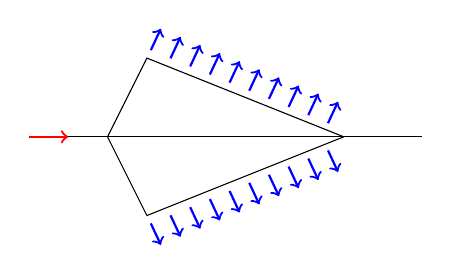
\begin{tikzpicture}
			\draw (-1,0) -- (4,0);
			\draw (0,0) -- (0.5,1) -- (3,0);
			\draw (0,0) -- (0.5,-1) -- (3,0);
			\draw[->, red, thick] (-1,0) -- (-0.5,0);
      \foreach \x in {0,1,...,9} {
        \draw[->,blue, thick] (0.55 + \x*0.25, 1.1 - \x*0.103)  --+ (65:0.3);
        \draw[->,blue, thick] (0.55 + \x*0.25, -1.1 + \x*0.103) --+ (-65:0.3);
      }
		\end{tikzpicture}
	\caption{Cherenkov radiation}
	\label{fig:label}
\end{figure}

\begin{align}
    x_p &= v_{p}\cdot t = \beta c t \nonumber \\
    x_{\text{em}} &= v_{\text{em}}\cdot t=\frac{c}{n}t \nonumber \\
    \cos\theta &= \frac{x_{\text{p}}}{x_{\text{em}}} = \frac{\frac{c}{n}t}{\beta c t} = \frac{1}{n\beta} \nonumber
\end{align}

which is independent from the angle \( \theta \).
% section cherenkov_radiation (end)

\section{Hough Transform} % (fold)
\label{sec:hough_transform}

The Hough-Transform is a feature extraction technique used in image analysis, computer vision and digital image processing.

the purpose is to find imperfect instances of objects within a certain cass of shapes by a voting procedure. This voting procedure is carried out in a parameter space from which object candidates are obtained as local maxima in a so called accumlator space that is explicitly constructed by the algorithm for computing the Hough-Transform.

Initially the Hough-Transform was concerned with finding straight lines but has been extended to identifying positions of arbitrary shapes, such as circles and ellipses.

\subsection{Linear Hough Transform} % (fold)
\label{sub:linear_hough_transform}

A linear function is normally defined as the following:

\[
  f(x) = m\cdot x + b
\]
where $m$ is the slope of the line and $b$ the intercept. For the Hough-Transform however, this representation is not ideal. For a vertical line $m$ would go to infinity which gives us an unbound transform space for $m$. For this reason Duda and Hart suggested the $\rho\text{-}\theta$ parametrization \parencite{Duda:1972}.

\[
  r = x\cos\theta + y\sin\theta
\]
where $r$ is the distance from the origin to the closest point in the line and $\theta$ is the angle between the $x$-axis and the line connecting the origin with that closest point.

\begin{figure}[h]
  \centering
  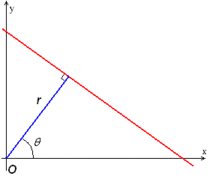
\includegraphics[width=0.3\textwidth]{pics/R_theta_line.png}
  \caption{$\rho\text{-}\theta$ parametrisation}
  \label{fig:rhotheta}
\end{figure}
% subsection linear_hough_transform (end)

This means given a single point in the plane, the set of all lines going through this point form a sinusoidal curve in $\rho\text{-}\theta$ space. Another point 
that lies on the same straight line in the plane will produce a sinusoidal curve that intersects with the other at ($\rho\text{-}\theta$).

\subsubsection{Example of a Linear HT} % (fold)
\label{ssub:example_of_a_linear_ht}

\begin{tikzpicture}
  \draw[<->] (3,0) -- (0,0) -- (0,3);

  \foreach \x in {0,0.5,1} {
    \draw[fill] (2-\x, 2-\x) circle (1pt);
  }
\end{tikzpicture}
\begin{table}
\centering
\caption{Angle vs Distance}
\begin{tabular}{rr}
\toprule
 Angle & Distance \\
\midrule
0 & 2.334 \\
\bottomrule
\end{tabular}
\end{table}

% subsubsection example_of_a_linear_ht (end)


\subsection{Circle Hough Transform} % (fold)
\label{sub:circle_hough_transform}

For this thesis we are interested in circle detection so we need to adapt our linear Hough Transform in order to find circles. In a two dimensional space, a circle can be described by:

\begin{equation}
		(x-c_x)^2 + (y-c_y)^2 = r^2
\end{equation}

Where $(c_x,c_y)$ is the center of the circle and $r$ the radius. The possible parameters for the parameters space are now $c_x, c_y$ and $r$. This means if we know the center of the circle the parameter space is one-dimensional and if we know the radius of the circle our parameter space is two-dimensional and of course if we know nothing the parameter space is three-dimensional.

% subsection circle_hough_transform (end)

\subsection{Combinatorial Approach} % (fold)
\label{sub:combinatorial_approach}

This approach is slightly different from the usual Hough Transforms. In this approach we use the fact that a circle is uniquely defined by 3 points.

% subsection combinatorial_approach (end)
% section hough_transform (end)


\chapter{Methods}

\section{Conventional Hough-Transforms} % (fold)
\label{sec:conventional_hough_transforms}

In the following subsections we discuss the conventional Hough-Transforms for the case of a one, two and three dimensional parameter space. These
methods were mainly considered to get an idea what was possible with the conventional hough transform. For closer study the method of choice was
the combinatorial approach briefly mentioned in subsection \ref{sub:combinatorial_approach} and discussed in depth in section \ref{sec:combinatorial_approach}
% section conventional_hough_transforms (end)

\subsection{1D: Known Center - Find Radius} % (fold)
\label{sub:1d_known_center_find_radius}

In this case the center(s) of the circle(s) is/are known so only the radius is missing. For the radius there is an array with a minimum value
and increasing by a defined stepsize to the maximum possible radius value. For the example in this thesis the minimum is $0$, the maximum radius
is $1$ and stepsize equal to $0.001$. Introducing following scoring function $\eta(r)$ allows to find the right radius.

\begin{equation}
  \eta(r) = (c_x - x)^2 + (c_y - y) - r ^ 2
\end{equation}

and using this in a gauss distribution

\begin{equation}
  w(\eta) = \frac{1}{\sqrt{2\pi}\sigma}\exp\left( \frac{-\eta^2}{2\sigma^2}\right)
\end{equation}
\begin{figure}[tb]
  \centering
  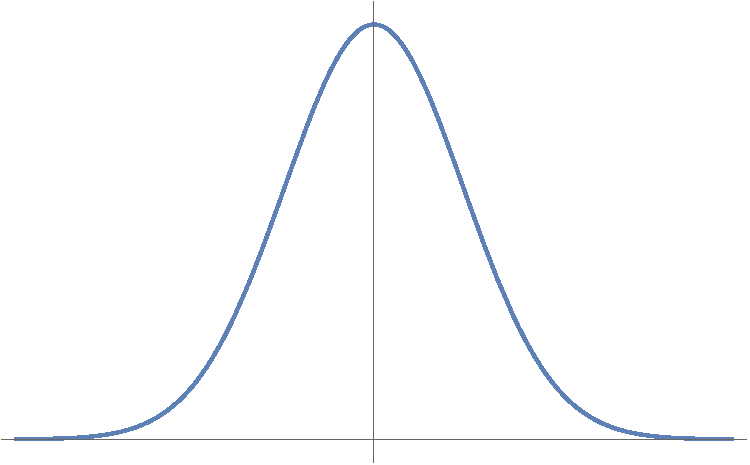
\includegraphics[width=0.5\textwidth]{pics/gauss}
  \caption{Using the probability density function of the normal distribution to calculate the score of a point in order to have a well defined maximum if a point
  lies directly on the circle and $\eta(r) = 0$. }
  \label{fig:gauss}
\end{figure}
This is of course just the circle equation with $c_x, c_y$ being the center of the circle, $x, y$ are the data points and $r$ the radius.
So if a lot of the data points have the same distance $r$ from the circle center there will be a high score for this particular radius. The index
for the highest score can then be used to find the corresponding radius.

\begin{figure}
  \begin{lstlisting}
  r = linspace(0,1,1001)
  for c in centers:
    scores = zeros(1001)
    for x,y in allPoints:
      s = 2*BIN_WIDTH
      eta = (c_x-x)**2 + (c_y-y)**2 - r**2
      scores += 1. / ( sqrt( 2 * Pi ) * s ) 
                 * exp( -( eta ** 2 ) 
                  / ( 2 * s ** 2 ) )
  
    index = max(scores)
    circle = {}
    circle['center'] = c
    circle['radius'] = r[index]
\end{lstlisting}
\caption{Pseudo code for the 1D Hough Transform. r is an array of length 1001 so $\eta$ will also be an array of length 1001. Scores is where the score for each iteration is stored. For each point the score is computed and added to the scores array and at the end the index with the highest score is the index we need to get the radius.}
\end{figure}



% subsection 1d_known_center_find_radius (end)
\subsection{2D: Known Radius - Find Center} % (fold)
\label{sub:2d_known_radius_find_center}



% section 2d_known_radius_find_center (end)

\subsection{3D: Nothing is Known - Find Everything} % (fold)
\label{sub:3d_nothing_is_known_find_everything}

% subsection 3d_nothing_is_known_find_everything (end)

\section{Combinatorial approach}
\label{sec:combinatorial_approach}
% The combinatorial approach relies on the fact that a circle is uniquely defined by 3 points. With 2 arbotrary points we couldn't tell which side the circle is
% going to go. A third point gives us all the information we need. The general idea then is the following:

\begin{enumerate}
\item Build all possible triples of points given the data points
\item For all the point triples calculate the center and the radius of the potential circle
\item Due to constraints in the radius many of the circles with a radius bigger than a certain threshold will be dropped.
\item Create a histogram with the radius distribution. Peaks in the radius distribution hint to a circle.
\item Scan the radius histogram for peaks and look at the center point histogram for the given radius of a peak. If there is also a peak in the center point histogram
      the set of the points of the triples lie on a circle with a radius and center given by the histogram peaks.
\end{enumerate}

\section{Calculating the Circle given 3 points}

Let $(A,B,C)$ be a triple of points in a 2D plane and $a,b,c$ the length of the sides opposite to the respective corner.
%
The semiperimeter is defined as
%
\begin{equation}
  s = \frac{a+b+c}{2}
\end{equation}
%
using this we can calculate the radius $R$ of the circumcircle of triangle $\overline{ABC}$:
\begin{equation}
  R = \frac{abc}{4\sqrt{s(a+b-s)(a+c-s)(b+c-s)}}
\end{equation}
We have $\lambda_1, \lambda_2, \lambda_3$ as the barycenteric coordinates of the circumcenter:
\begin{align}
  \lambda_1 &= a^2\cdot(b^2+c^2-a^2)\\
  \lambda_2 &= b^2\cdot(a^2+c^2-b^2)\\
  \lambda_3 &= c^2\cdot(a^2+b^2-c^2)
\end{align}
Multiplying a matrix consisting of the column vectors of $A,B,C$ with a column vector of $\lambda_1, \lambda_2, \lambda_3$ and dividing the resulting vector by the sum of the barycentric coordinates (for noramlization) leads to the circumcenter of the triangle $\overline{ABC}$ 
%
\begin{equation}
  \begin{pmatrix}
    A_x & B_x & C_x \\
    A_y & B_y & C_y
  \end{pmatrix} \cdot \begin{pmatrix}
    \lambda_1\\
    \lambda_2\\
    \lambda_3
  \end{pmatrix} = \boldsymbol{P'}
\end{equation}
%
\begin{equation}
  \frac{\boldsymbol{P'}}{\lambda_1+\lambda_2+\lambda_3} = \boldsymbol{P}
\end{equation}
%
\begin{figure}[tb]
\centering
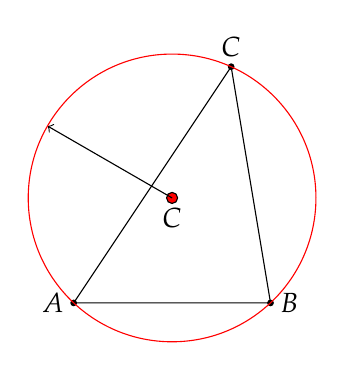
\begin{tikzpicture}
\coordinate (A) at (0,0);
\coordinate (B) at (2.5,0);
\coordinate (C) at (2,3);
\coordinate (Ci) at (1.25,1.33333);
\def\r{1.827}
\draw[thin] (A) -- (B) -- (C) -- cycle;
\node[left] at (A) {$A$};
\node[right] at (B) {$B$};
\node[above] at (C) {$C$};
\draw[fill=black] (A) circle (1pt);
\draw[fill=black] (B) circle (1pt);
\draw[fill=black] (C) circle (1pt);
\draw[fill=red] (Ci) circle (2pt) node [below] (Ci) {$C$};

\draw[->] (1.25,1.33333) -- +(150:1.827);
\draw[red] (1.25,1.33333) circle (1.827);
\end{tikzpicture}
\caption{The circumradius and the circumcenter of a circle defined by the points}
\label{fig:circum_fig}
\end{figure}

\subsection{Drawback}
	

There is also a drawback with this method:

\begin{itemize}
\item The combinatorics blow up with a high number of data points \( \binom{N}{3} \)
\end{itemize}

So for example with 200 data points (circle data and background) the number of triplets is

\[ \binom{200}{3} = 1313400 \]

and for 300:

\[ \binom{300}{3} = 4455100 \]


\begin{figure}[tb]
  \centering
  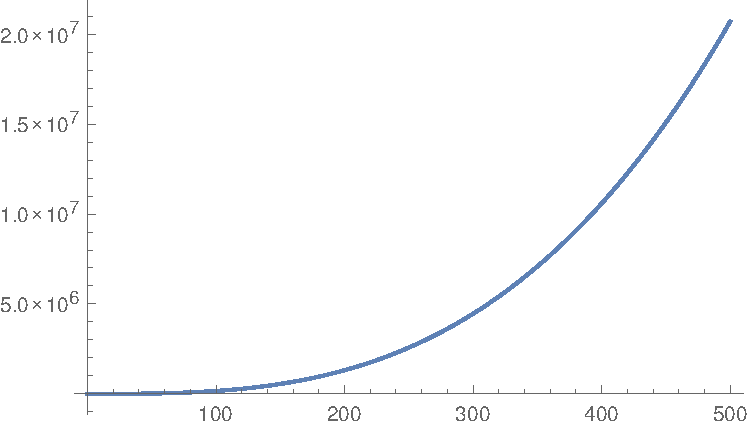
\includegraphics[width=0.5\textwidth]{pics/binomial_growth}
  \caption{Binomial Growth with $\binom{N}{3}$}
  \label{fig:figure1}
\end{figure}


\subsection{Average Radius of Random Circles In a Unit Square} % (fold)
\label{ssub:average_radius_of_random_circles_in_a_unit_square}

First we calculate the expected area of a triangle.

Let \( A = (a_1, a_2),\ B = (b_1, b_2),\ C = (c_1, c_2)\) be the vertices of the random triangle \( T \). We consider the case where \( a_2
> b_2 > c_2 \) which takes $\frac{1}{6}$ of the total ``Volume''. Fix \( a_2, b_2, c_2 \) for the moment and we can write.
\[
  b_2 = (1-t)a_2 + tc_2, \qquad 0 \leq t \leq 1.
\]
The side $AC$ of $T$ intersects the horizontal level $y=b_2$ at the point $S=(s,b_2)$ with
\begin{equation}
  s = s(a_1,c_1,t) = (1-t)a_1 + tc_1
\end{equation}
% subsubsection average_radius_of_random_circles_in_a_unit_square (end)
\chapter{Results}


\chapter{Conclusions} % (fold)
\label{cha:conclusions}

% chapter conclusions (end)

\printbibliography
\end{document}
